\chapter{电路设计与仿真}

本章对基于Cadence Virtuoso仿真软件和SMIC 0.18um BCD工艺设计的变换器芯片的各个关键电路进行分析和仿真,包括欠压锁定电路、内部供电电路、模式切换电路、退磁时间动态校准电路、峰值电流控制电路、精确谷底导通电路、谷值锁定电路、逻辑控制电路和各个保护电路等。最后对整体电路进行系统仿真,测试变换器芯片的基本功能,验证该电路设计的合理性和可靠性。

\section{欠压锁定电路}




\section{内部供电电路}

\subsection{带隙基准电路}

在变换器芯片工作过程中,其内部的各个模块都需要相应的偏置电压和偏置电流,为了维持这些偏置电压和偏置电流的精确和稳定性,不能用普通的与电源无关的基准电路产生全部的信号,因此需要设计带隙基准电路,提供受电源电压和温度变化影响很小的基准电压电流,使得变换器芯片适用于各种工况下。

带隙基准电路的实现原理是通过将一个正温度系数的电压和一个负温度系数的电压加权相加后,抵消掉其正负温度系数,得到不受温度变化影响的零温度系数的基准电压。实际电路中,负温度系数的电压利用双极型晶体管产生,其正向压降$V_{be}$带有负温度特性。通过半导体物理的基础知识可知,电压$V_{be}$的公式为:
\begin{equation}
    \label{eq:Vbe公式}
    V_{be} = V_T \cdot ln(\frac{I_c}{I_s})
\end{equation}
其中,$V_T$是热电压,公式为:
\begin{equation}
    \label{eq:VT公式}
    V_T=\frac{kT}{q}
\end{equation}
$I_c$是PN结的集电极电流,公式为:
\begin{equation}
    \label{eq:Ic公式}
    I_c=I_s \cdot exp(\frac{V_{be}}{V_T})
\end{equation}
$I_s$是PN结饱和电流,公式为:
\begin{equation}
    \label{eq:Is公式}
    I_s=bT^{4+m} exp\frac{-E_g}{kT}
\end{equation}
结合式\eqref{eq:Vbe公式}、\eqref{eq:Ic公式}和\eqref{eq:Is公式},通过正向压降$V_{be}$对温度求偏导,可计算得$V_{be}$的负温度系数公式:
\begin{equation}
    \label{eq:Vbe/T公式}
    \frac{\partial V_{be}}{\partial T} = \frac{ V_{be} - (4+m)V_T - E_g/q}{T}
\end{equation}

正温度系数的电压同样可以通过双极型晶体管来产生,不同电流密度的电流流经晶体管会产生不同的负温度系数,两者的差值电压$\varDelta V_{be}$带有正温度系数。实际电路中为了满足晶体管的匹配性,使用两个不同面积的双极型晶体管来产生不同电流密度的作用。令两个双极型晶体管的面积比为$1:N$,则流经单个晶体管的电流密度比N:1,可计算得晶体管压差$\varDelta V_{be}$的公式为:
\begin{equation}
    \label{eq:△Vbe公式}
    \varDelta V_{be} = V_T ln(\frac{I_c}{I_s}) - V_T ln(\frac{I_c}{nI_s}) = V_T \cdot ln(n)
\end{equation}
通过$\varDelta V_{be}$对温度求偏导可计算得正的温度系数公式:
\begin{equation}
    \label{eq:△Vbe/T公式}
    \frac{\partial \varDelta V_{be}}{\partial T} = \frac{k}{q}\cdot ln(n)
\end{equation}


由式\eqref{eq:Vbe/T公式}和\eqref{eq:△Vbe/T公式}计算可知,在常温T=300K的条件下,当$V_{be}\thickapprox $ 750 mV时,$V_{be}$的负温度系数约等于-1.5 mV/K,$\varDelta V_{be}$的正温度系数为0.087ln(n) mV/K。为了合理地产生零温度系数电压,防止双极型晶体管的面积太大,需对正负温度系数加权相加可得。

为了满足变换器芯片中的低压数字模块,



\subsection{高压LDO电路}

由辅助绕组产生的供电端电压对于片内的元器件而已电压过大且不够稳定,无法直接用于作为供电电压,需要设计用于产生稳定输出电压的低压线性稳压器电路,将供电端的高压转化为可为内部电路供电的电源电压输出。
\begin{figure}[htbp] 
    \centering
    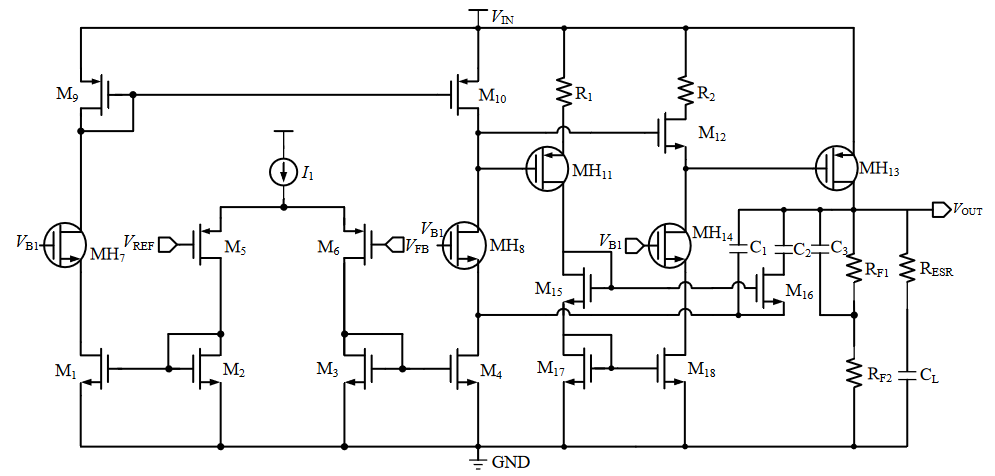
\includegraphics[width=0.6\linewidth]{figures/高压LDO.png}
    \caption{高压LDO电路图}
    \label{fig:高压LDO}
\end{figure}

本文设计的高压LDO电路如图~\ref{fig:高压LDO}所示,该电路


%\section{抖频振荡器}

%\section{模式切换电路}

%\section{退磁时间动态校准电路}

\section{峰值电流控制电路}
\label{sec:峰值电流控制电路}
%为了防止出现如前文~\ref{sec:多模式切换}小节中提到的峰值电流和开关频率同时变化引起的相位裕度降低和电路不稳定情况,轻载时采取的RVS工作模式通过改变开关频率的方式维持峰值电流的基本恒定。副边反馈引脚电压信号$V_{FB}$如~\ref{sec:峰值电流控制电路}小节中提到的,是峰值电流参考电压$V_{CSP}$的重要组成部分,可以一定程度地反映输出负载电流的大小。当负载电流突然增大时,为了满足变大的输出功率,变压器原边需要增大高边功率管的导通时间提供更多的能量给输出电容,因此$V_{CSP}$增大,$V_{FB}$也相应地增大;当负载电流突然减小时,同理$V_{FB}$也会相应地减小。同时为了降低导通损耗,需要维持一个较低的峰值电流,因此在负载波动时,利用谷值锁定电路通过随$V_{FB}$变化动态调节谐振谷的数量,改变$T_w$时间长度的方式改变开关频率,更快地恢复输出电压的稳定。

%\section{前沿消隐电路}



\section{精确谷底导通电路}

根据上文3.6.2节介绍的精确谷底导通技术,本小节对图~\ref{fig:精确谷底导通技术框图}中的精确谷底导通模块进行具体的描述并仿真其基本功能。

图~\ref{fig:精确谷底导通电路图1}是精确谷底导通模块的电路框图。包括两个峰值检测电路、压控高通滤波器、SR锁存器、鉴相鉴频器、电荷泵和逻辑电路等。

\begin{figure}[htbp] 
    \centering
    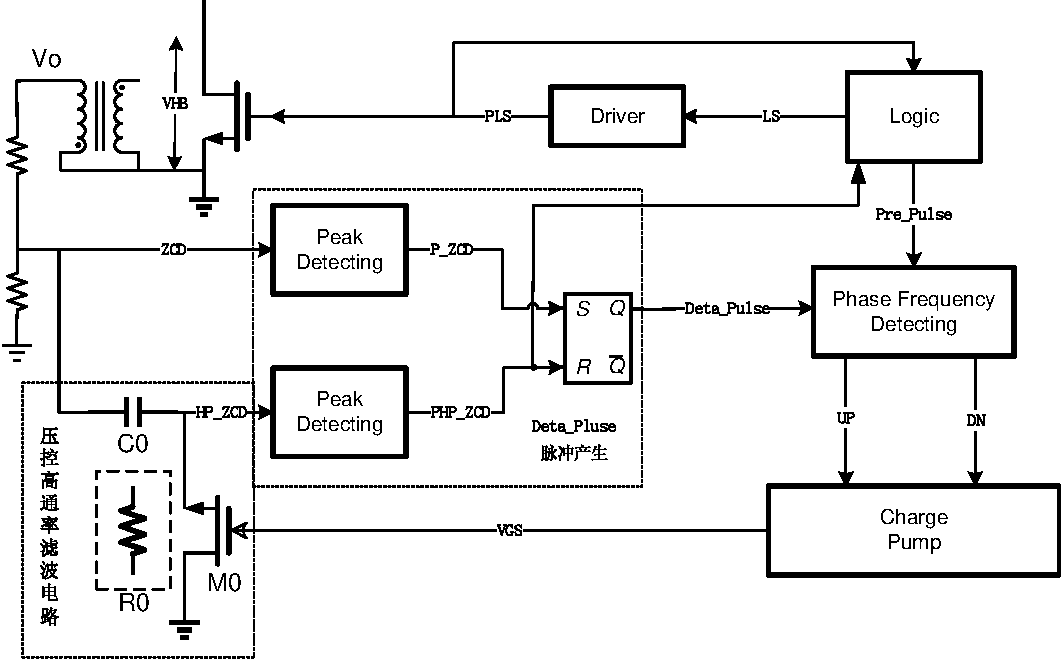
\includegraphics[width=0.8\linewidth]{figures/精确谷底导通电路图1.pdf}
    \caption{精确谷底导通电路图1}
    \label{fig:精确谷底导通电路图1}
\end{figure}


因为功率管半桥节点信号$V_{HB}$的电压值过大,无法直接输入变换器芯片内进行处理,因此对在等待时间$T_w$内同样带有谐振信息的辅助绕组分压引脚ZCD的电压信号$V_{ZCD}$进行采样处理。由于$V_{ZCD}$信号和$V_{HB}$信号的谐振电压相位相反,故$V_{HB}$的谐振谷底对应$V_{ZCD}$的谐振谷峰值。如图~\ref{fig:精确谷底导通电路图1}中所示,采用峰值检测电路来检测$V_{ZCD}$信号在等待时间$T_w$内的谐振谷峰值,并输出对应的峰值脉冲信号P\_ZCD。

峰值检测电路图如图~\ref{fig:峰值检测电路图}所示。峰值检测电路包括一个由晶体管M2、M4、M5、M6和M7组成的五管运算放大器,一个晶体管M9和M10组成的电流镜以及晶体管M11构成的源极跟随器。电流镜晶体管M12为源极跟随器M11提供偏置电流。该电路的工作原理是通过运算放大器比较输入电压$V_{in}$和输出电压$V_{out}$的大小,当输入电压$V_{in}$大于输出电压$V_{out}$时,运算放大器输出低电平,拉低电流镜晶体管M9的栅端电压,电流镜开始工作,对电容$C_1$进行充电,电压$V_1$逐渐升高,$V_{out}$在源极跟随器的作用下也逐渐增大,跟随$V_{in}$变化。当$V_{in}$不再增大,$V_{in}$开始小于$V_{out}$时,运算放大器输出高电平,拉高电流镜晶体管M9的栅端电压,电流镜停止工作,不再给电容$C_1$进行充电,进而输出电压$V_{out}$也保持不变,实现峰值检测的功能。最后通过一个脉冲产生电路输出峰值脉冲信号。同时为了检测在电路在不同周期内不同大小的输入电压$V_{in}$,加入复位开关管M13,当接收到复位信号$R_{st}$后,开关管M13导通,对电容$C_1$进行放电,实现复位的功能。

\begin{figure}[htbp] 
    \centering
    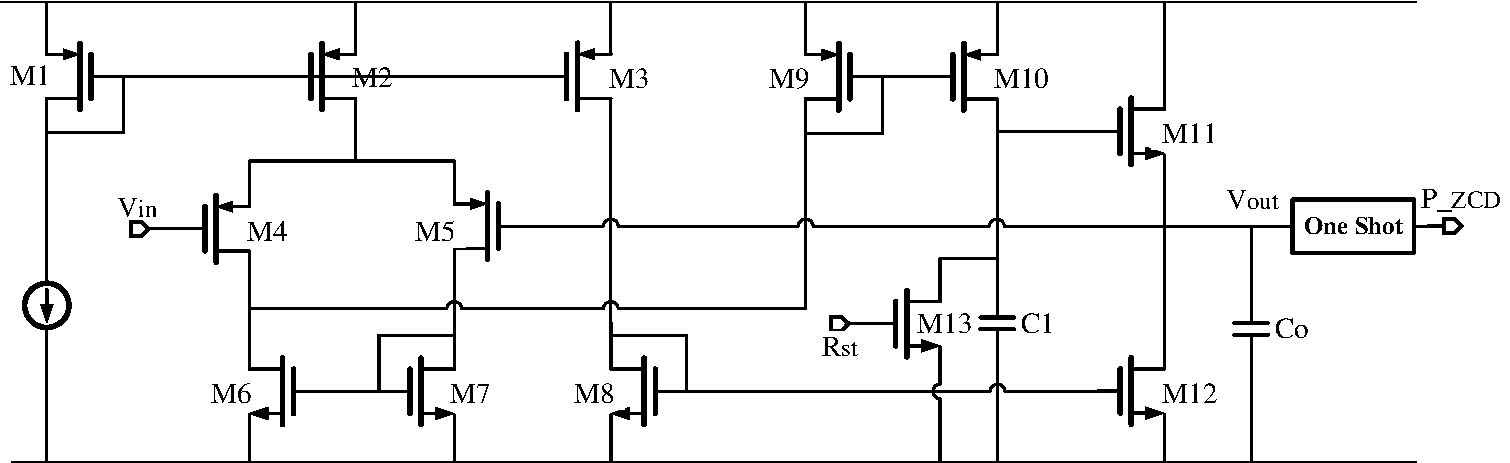
\includegraphics[width=1.0\linewidth]{figures/峰值检测电路图.pdf}
    \caption{峰值检测电路图}
    \label{fig:峰值检测电路图}
\end{figure}

由于驱动电路等电路结构对逻辑控制信号存在延时问题,为了满足精确的谷底导通功能,不能直接将信号$V_{ZCD}$通过峰值检测电路产生的峰值脉冲信号P\_ZCD直接作为时钟信号CLK输入到逻辑控制模块来产生下个开关周期的逻辑控制信号LS。针对于该问题,新颖性地提出了迫使精确谷底导通模块在$V_{HB}$谐振谷底到达之前产生低边功率管的导通时钟信号CLK的方案,使得逻辑控制信号LS通过驱动电路延时后,输出的栅极驱动信号LSGD恰好位于$V_{HB}$信号谐振谷底的位置处,此时导通低边功率管,不仅降低开关损耗,还可以极大地减小峰值检测电压的过冲现象。为满足该功能,要求逻辑控制信号LS超前产生的时间近似等于驱动电路等结构的延时时间。

该模块中实现超前采样$V_{ZCD}$信号峰值的核心电路是采用的压控高通滤波器电路,如图~\ref{fig:精确谷底导通电路图1}中所示,可以通过控制MOS管的栅极电压$V_{GS}$来调节MOS管的导通电阻$R_{on}$,$R_{on}$的计算公式为:
\begin{equation}
    \label{eq:Ron公式}
    R_{on}=\frac{1}{\mu_n C_{ox} \frac{W}{L} (V_{GS} - V_{TH})}
\end{equation}
由式可知,随着MOS管栅极电压$V_{GS}$的增大,其导通电阻逐渐减小。根据高通滤波器的幅频曲线公式可知,当功率管栅压$V_{GS}$为零电压时,功率管截止,导通电阻近似无穷大,对应的时间常数RC无穷大,相位变化为0度,压控高通滤波器的输出信号$V_{ZCD,PH}$和信号$V_{ZCD}$的电压波形重合。随着栅压信号$V_{GS}$的增大,时间RC常数越小,$V_{ZCD,PH}$波形超前的相位变化越大,直至时间常数RC等于零时,超前相位最大值90度。
\begin{equation}
    \label{eq:jw公式}
    \varphi_{j\omega }=\arctan (\frac{\omega_c}{j\omega R C })
\end{equation}
其中$\omega_c$为滤波器的截止频率。通过和合理的调节MOS管栅压信号$V_{GS}$的值,即可调节$V_{ZCD,ph}$波形恰好超前$V_{ZCD}$电压波形的相位时间信号D\_Phase和驱动电路的延时时间信号L\_Phase的脉冲宽度相等,实现低边功率管栅极驱动信号的精确谷底导通功能。其中,如图~\ref{fig:精确谷底导通电路图1},信号D\_Phase是信号$V_{ZCD,PH}$和$V_{ZCD}$通过峰值采样电路分别输出的峰值脉冲信号PH\_ZCD与P\_ZCD经过一个SR锁存器产生的;信号L\_Phase则是将栅极驱动信号LSGD经过电平移位器降为低压后同逻辑控制信号LS经过SR锁存器产生的。

压控高通滤波器的栅压信号$V_{GS}$的调控方式采用了锁相环电路中的鉴相鉴频器和电荷泵结构来动态调节实现。图~\ref{fig:鉴相鉴频器电路图}为该模块使用的鉴相鉴频器电路和电荷泵的电路图。包括两个带复位端的下降沿D触发器和一个与门组成。触发器的D输入端都接高电平保持逻辑"1",触发器1的时钟输入端D\_Phase是信号$V_{ZCD,PH}$和信号$V_{ZCD}$波形的超前相位时间差;触发器2的时钟输入端L\_Phase是逻辑控制信号LS和栅压驱动信号LSGD的延迟时间差。通过这两个D触发器检测D\_Phase和L\_Phase信号的相位时间差信号UP和DN,再通过信号UP和DN控制电荷泵的开关S1和S2,选择对电容$C_{GS}$进行充电或放电功能。

\begin{figure}[htbp] 
    \centering
    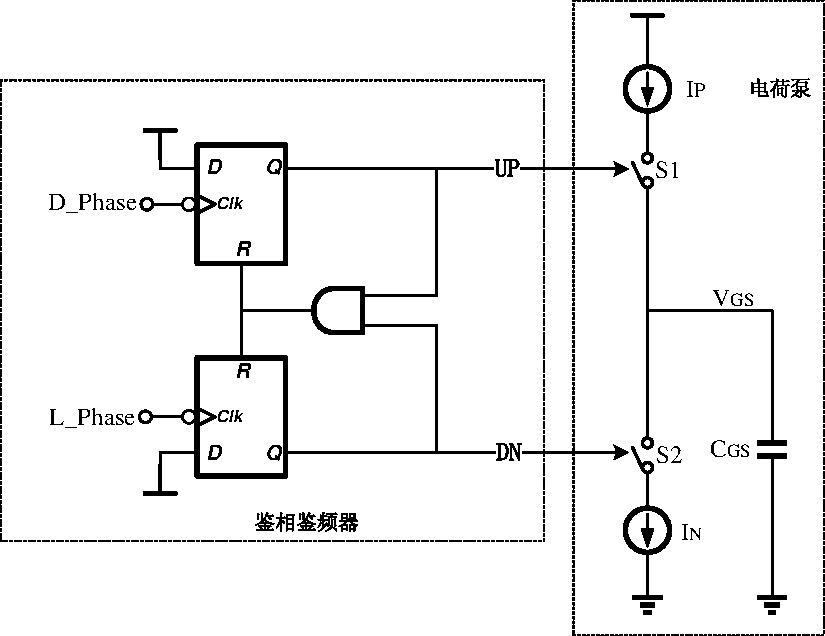
\includegraphics[width=0.6\linewidth]{figures/鉴相鉴频器.pdf}
    \caption{鉴相鉴频器和电荷泵电路图}
    \label{fig:鉴相鉴频器电路图}
\end{figure}

鉴相鉴频器和电荷的波形图如~\ref{fig:鉴相鉴频器波形图}所示。不同于上升沿D触发器组成的鉴相鉴频器,该模块中使用的下降沿鉴相鉴频器的输出信号UP和DN是信号D\_Phase和L\_Phase的下降沿的相位时间差。当信号D\_Phase先于信号L\_Phase变为低电平时,信号UP由低变高,导通开关S1,电流源$I_P$对电容$C_{GS}$进行充电,电压$V_{GS}$逐渐增大;当信号L\_Phase的下降沿到来后,UP由高变低,开关S1关断,$V_{GS}$保持不变。同理,信号DN和UP相似,区别在于L\_Phase先于信号D\_Phase变为低电平时有低变高,导通开关S2通过电流源$I_N$对电容$C_{GS}$进行放电,电压$V_{GS}$逐渐减小。随着鉴相鉴频器和电荷泵电路的不断工作,最终信号D\_Phase和信号L\_Phase几乎重叠,信号UP和DN脉冲保持一致,同时给电容$C_{GS}$进行充电和放电,电压$V_{GS}$维持稳定。

\begin{figure}[htbp] 
    \centering
    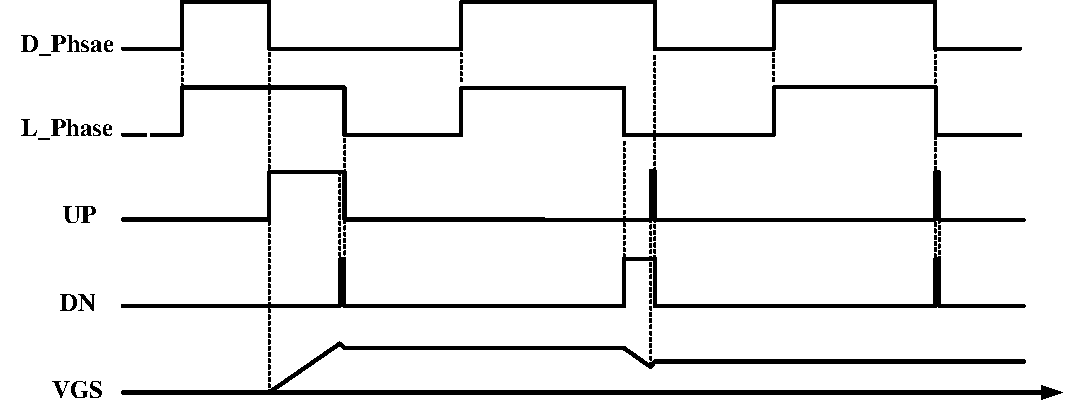
\includegraphics[width=0.8\linewidth]{figures/鉴相鉴频器波形图.pdf}
    \caption{鉴相鉴频器电荷泵波形图}
    \label{fig:鉴相鉴频器波形图}
\end{figure} 

其中,模块中使用的单端结构电荷泵的实际电路图如图~\ref{fig:电荷泵电路图}所示,电荷泵的单端结构占用面积较小,且更易于设计,满足于精确谷底导通模块的使用需求。同时为了减小电荷泵电路中的电荷注入、时钟馈通和电荷共享的非理性效应,采用了源极开关型结构。该电荷泵结构未直接将MOS开关管MP5、MN4连接在电容$C_{GS}$的上极板,通过电流镜晶体管MP6、MN3将开光管和电容隔离开,阻挡了开关管关断时反型层中的沟道电荷注入电容,提高了电压$V_{GS}$的稳定性。

\begin{figure}[htbp] 
    \centering
    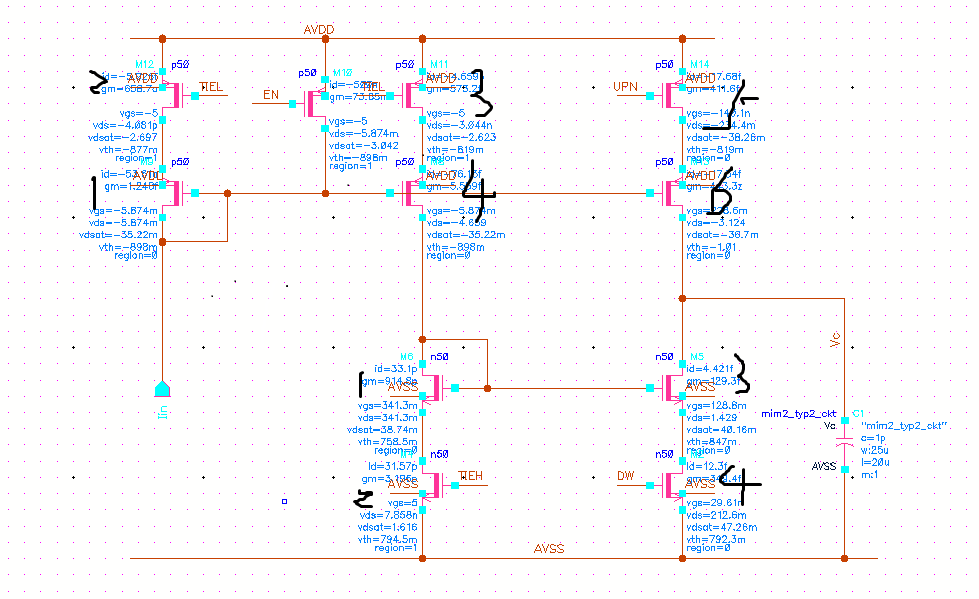
\includegraphics[width=0.8\linewidth]{figures/电荷泵电路图.png}
    \caption{电荷泵电路图}
    \label{fig:电荷泵电路图}
\end{figure} 

为了满足PMOS管在信号UP的控制下正确地导通和关断,通过一个反相器输出信号UPN来控制开关管MP5,在信号UP电压由低变高时,信号UPN电压由高变低,导通开关管MP5,对电容$C_{GS}$进行充电;信号DN电压由低变高时,直接控制开关管MN4导通,对电容$C_{GS}$进行放电。电荷泵电路除了由晶体管MP1、MP4、MP6组成的PMOS电流镜和晶体管MN1、MN3组成的NMOS电流镜,还额外加入了晶体管MP2、MP3、MN2来和开关管MP5 MN4相对应,提高了电路的对称性,在开关管导通时使得电流镜晶体管的源极电压相等,提高电流镜的复制比精度,迫使电容$C_{GS}$的充放电电流尽可能一致。


结合图~\ref{fig:精确谷底导通波形图}中的工作波形,精确谷底导通模块的具体工作过程为:当工作模式首次切换为RVS模式时,此时压控高通滤波器的栅压$V_{GS}$为零,晶体管M0未导通,晶体管的导通电阻近似无穷大,高通滤波器的相位变化为零,信号$V_{ZCD,PH}$和信号$V_{ZCD}$波形重叠,模块将峰值检测电路检测的$V_{ZCD}$峰值脉冲信号P\_ZCD作为时钟CLK输出给逻辑控制模块,产生的逻辑控制信号LS在t1时刻的$V_{HB}$谐振谷底处由低电平变为高电平,经过驱动电路延时后,栅极驱动信号在t2时刻控制低边功率管导通,此时$V_{HB}$电压较大,产生较大的开关损耗。信号D\_Phase和L\_Phase经过鉴相鉴频器输出的信号UP导通电荷泵开关管对电容充电,压控高通滤波器栅压$V_{GS}$线性增大。

\begin{figure}[htbp] 
    \centering
    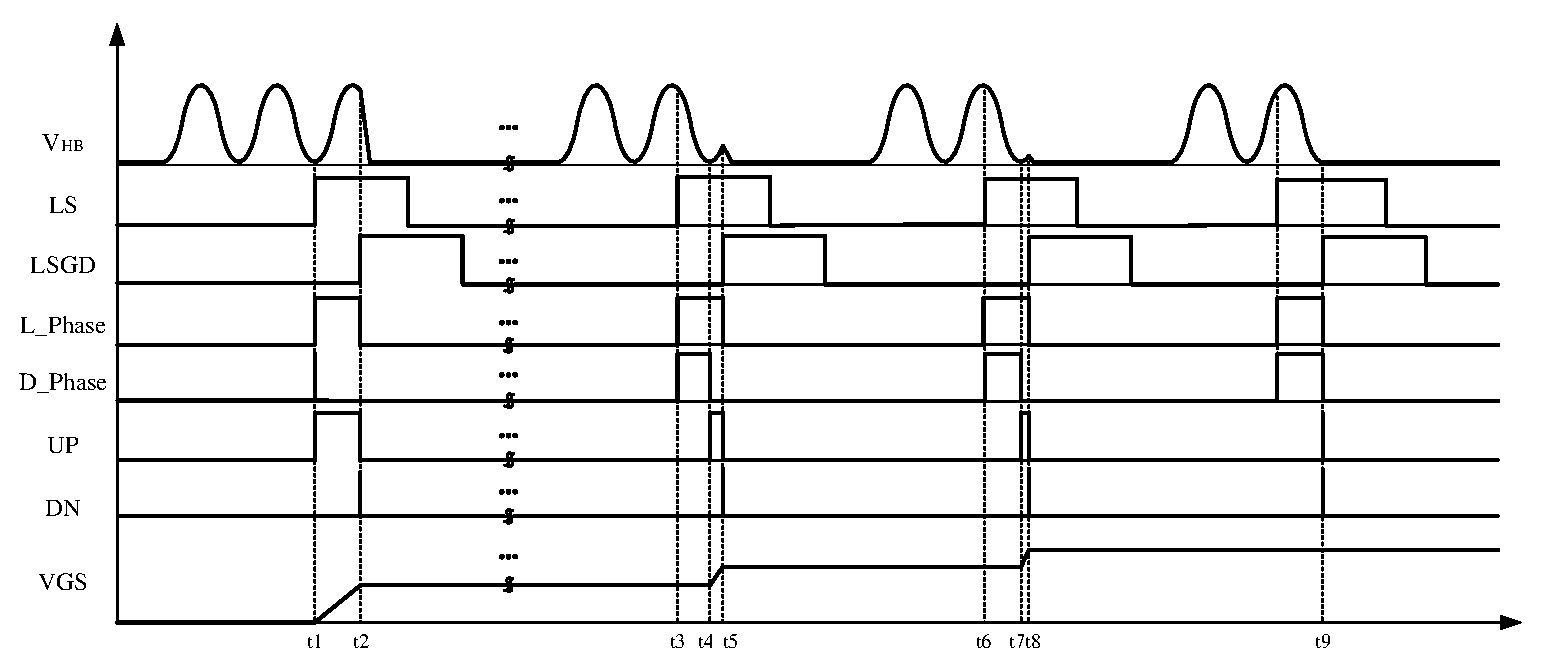
\includegraphics[width=1.0\linewidth]{figures/精确谷底导通波形图.pdf}
    \caption{精确谷底导通电路相关波形图}
    \label{fig:精确谷底导通波形图}
\end{figure} 

经过几个开关周期的充电后,栅压$V_{GS}$大于晶体管M0阈值电压,晶体管导通,压控高通滤波器产生的超前信号D\_Phase迫使信号LS在$V_{HB}$谐振谷底前导通,与信号L\_Phase之间的相位差UP也相应减小,成功实现逐步逼近功能,栅极驱动信号LSGD在t5时刻导通低边功率管,此时虽仍未在谷底处导通,但开关损耗已大大降低。

最后经过几个开关周期的变化,压控高通滤波器产生的超前信号D\_Phase几乎与信号L\_Phase重叠,鉴相鉴频器输出信号UP和DN脉冲宽度相等,电容上电压$V_{GS}$维持稳定,t9时刻LSGD在$V_{HB}$谐振谷底处实现精确导通低边功率管的功能。

\begin{figure}[htbp] 
    \centering
    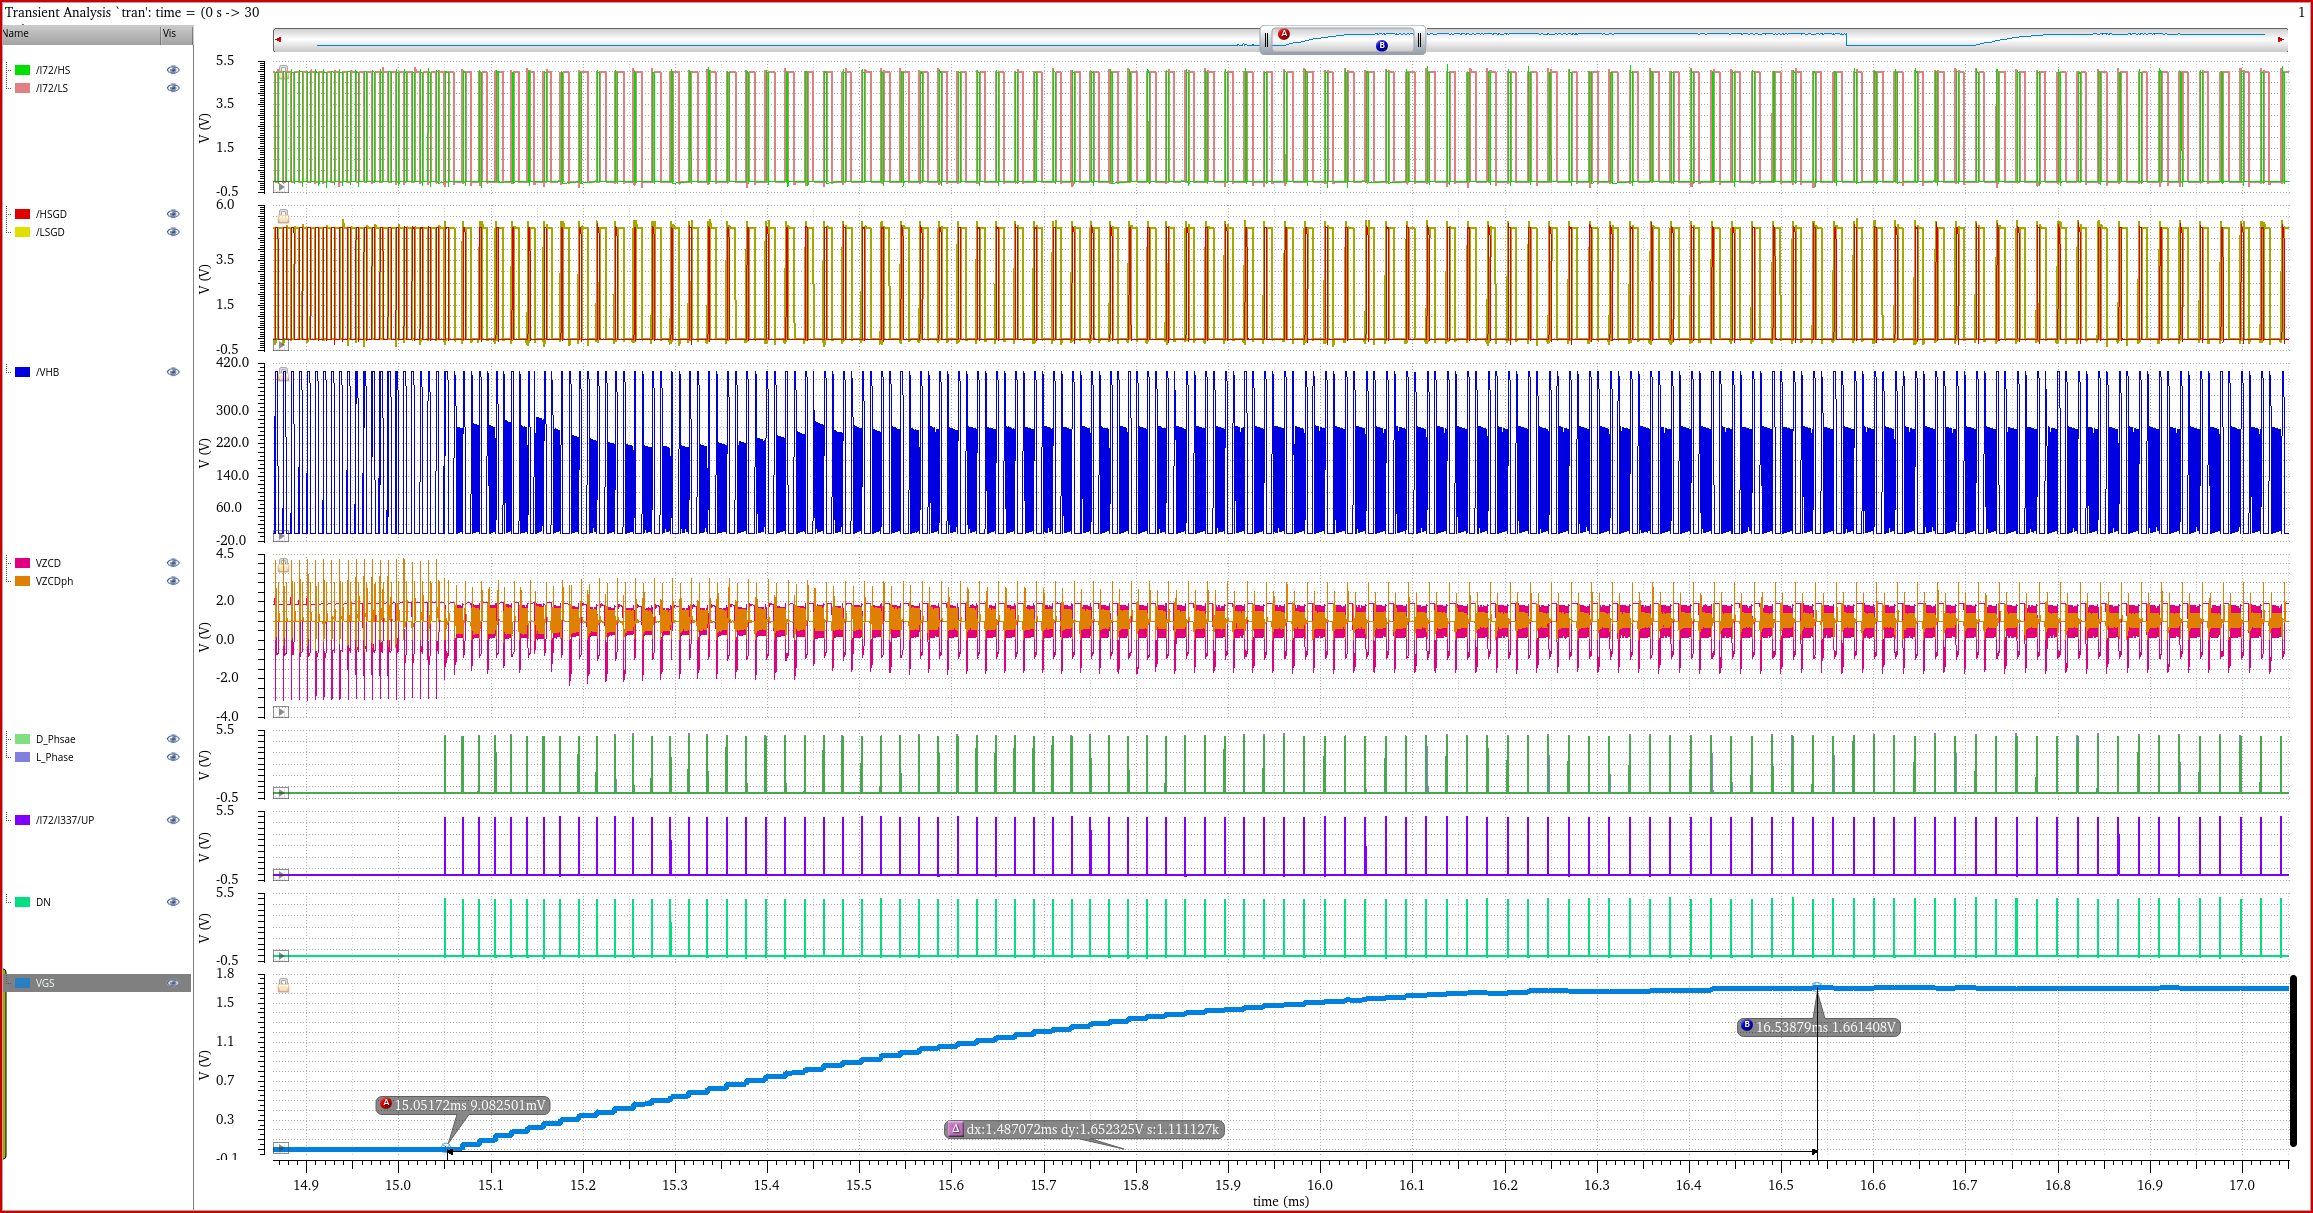
\includegraphics[width=0.8\linewidth]{figures/valley_switch.png}
    \caption{精确谷底导通电路相关波形仿真图}
    \label{fig:谷底导通仿真图}
\end{figure} 


\begin{figure}[htbp]
	\centering
	\subcaptionbox{未稳定\label{fig:谷底导通仿真图1}}{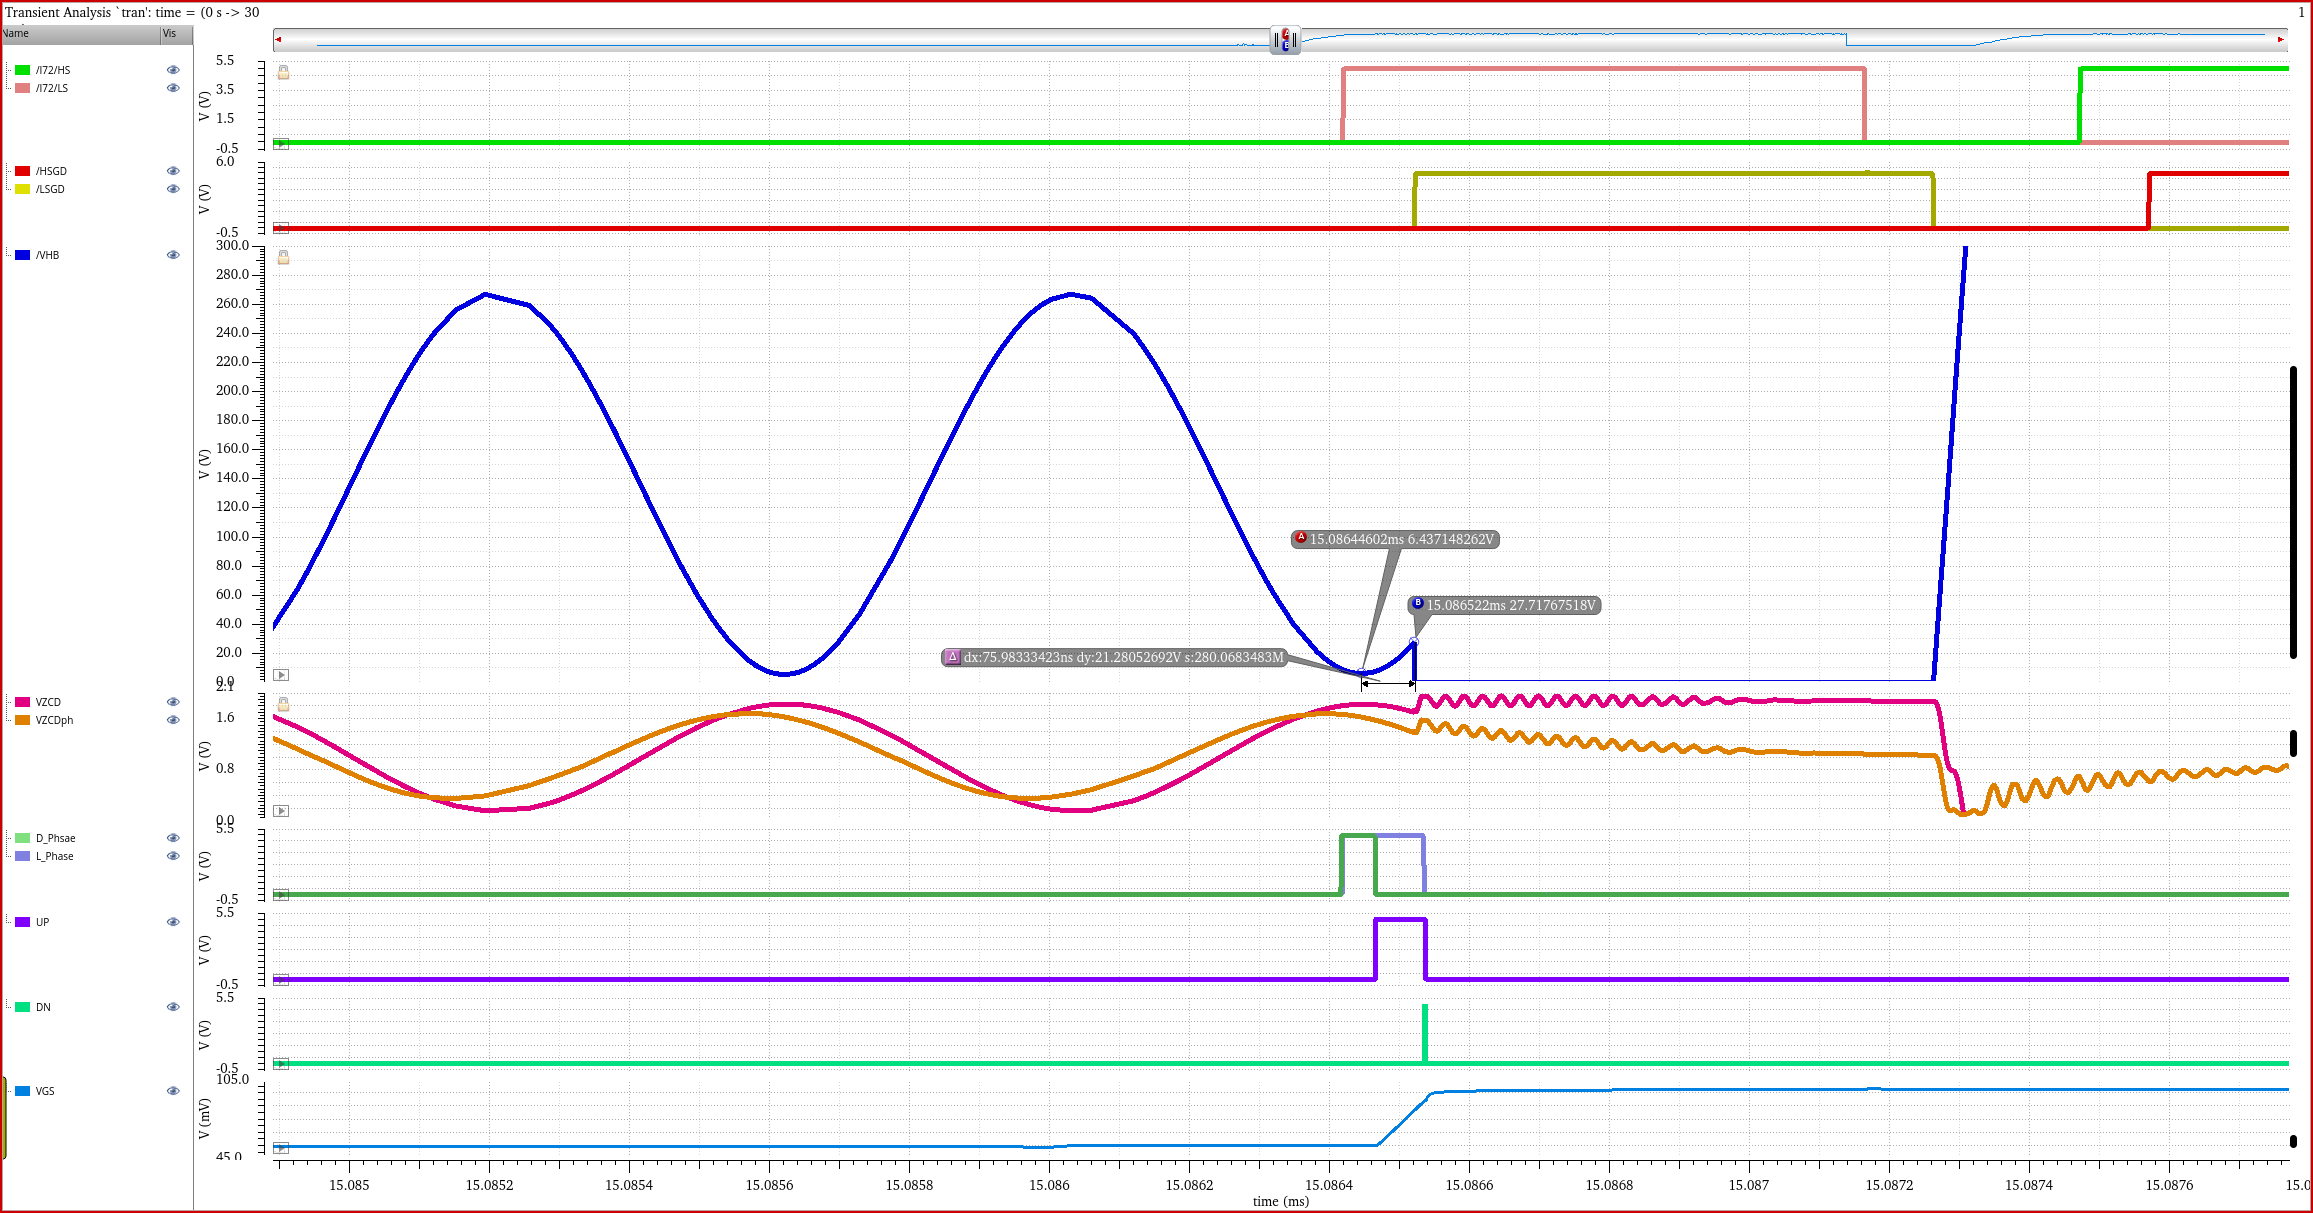
\includegraphics[width = 0.45\linewidth]{figures/valley_switch1.png}}
	\subcaptionbox{稳定\label{fig:谷底导通仿真图2}}{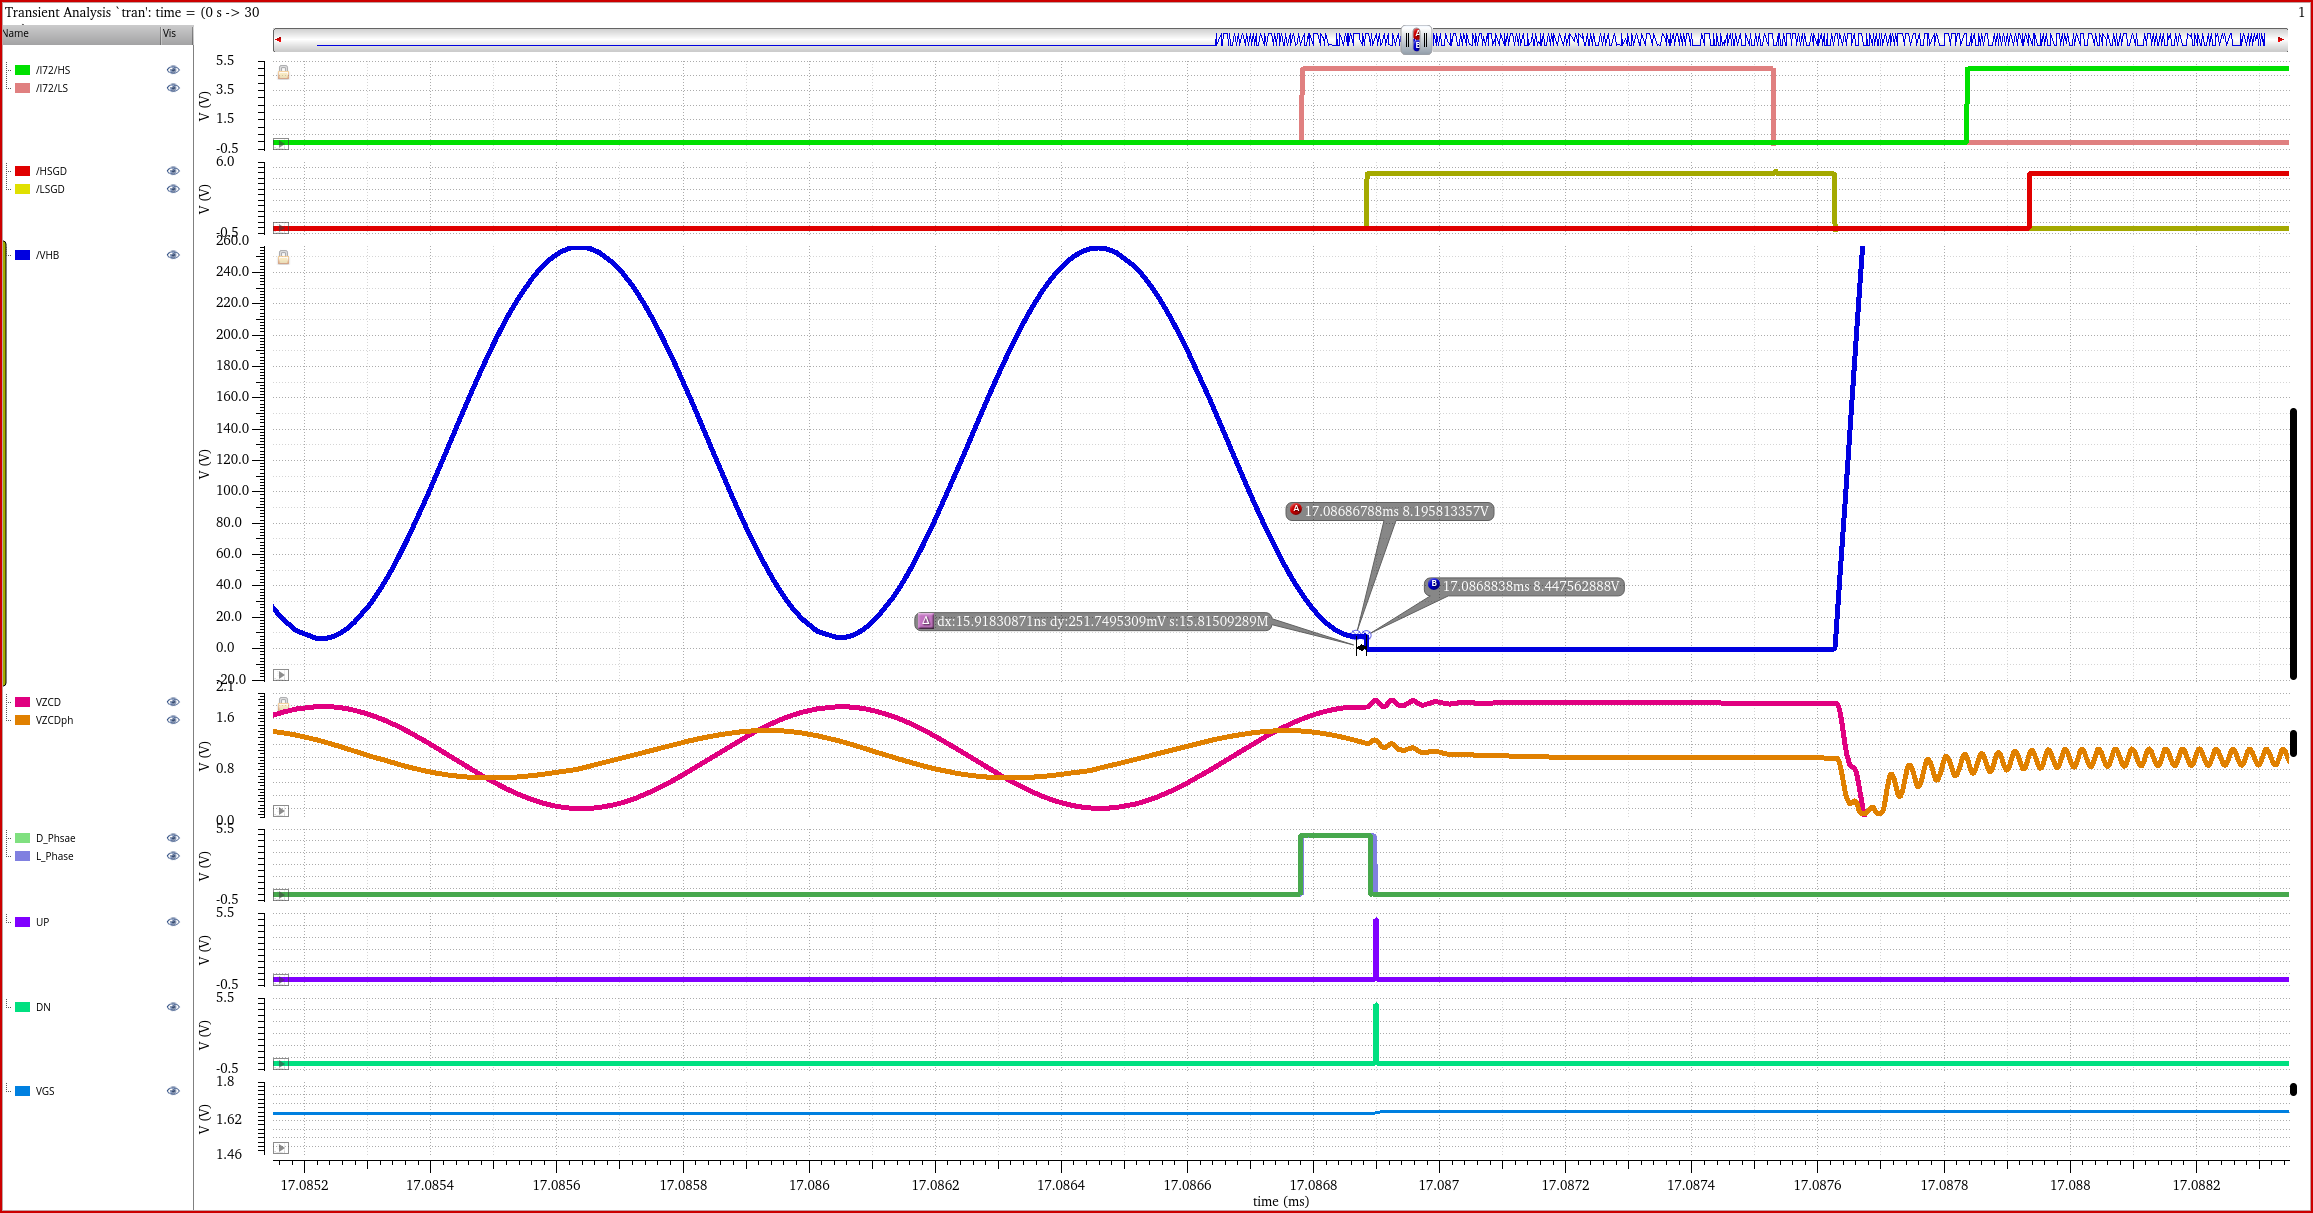
\includegraphics[width = 0.45\linewidth]{figures/valley_switch2.png}}
	\caption{谷底导通放大仿真图}
	\label{fig:谷底导通放大仿真图}
\end{figure}

图~\ref{fig:谷底导通仿真图}为精确谷底导通电路相关波形仿真图,由仿真图可见,当系统由恒流模式切换为恒压模式中的RVS工作模式后,精确谷底导通模块内压控高通滤波器的栅压$V_{GS}$随着开关周期逐渐增大,经过1.43ms后稳定在1.65V,此时电路已完成精确谷底导通功能。图~\ref{fig:谷底导通放大仿真图}中分别展示了电路在栅压$V_{GS}$未稳定和稳定后的具体波形图。在图~\ref{fig:谷底导通放大仿真图} (a)中,栅极驱动信号LSGD未能在$V_{HB}$谐振谷底处导通,其导通时刻$V_{HB}$电压值等于27.7V,和谷底处电压值的差值约为21.3V。在图~\ref{fig:谷底导通放大仿真图} (b)中可见,由于电路精度的限制,栅极驱动信号LSGD导通低边功率管时$V_{HB}$电压值和谷底电压值的差值仅为252mV,可以近似忽略不计,实现了电路的设计需求和功能。

%通过逻辑控制电路得到LS和PLS信号的延时时间Pre\_Pulse。为了预判谷底信号,通过一个使用MOS管充当电阻的压控高通滤波器电路,产生$V_{ZCD}$对应的超前时间信号VHP\_ZCD,只需适当的调节VGS的大小即可控制VHP\_ZCD信号的超前时间大小。分别使用两个峰值检测电路来检测并得到两个信号的峰值脉冲信号,经过SR锁存器产生超前时间Deta\_Pulse。为了轻微的调节栅极电压信号VGS,使用了PLL电路中的鉴相鉴频器和电荷泵电路来控制Deta\_Pulse信号逐步逼近Pre\_Pulse信号,完成低边功率管的精确谷底导通功能。




\section{谷值锁定电路}

在RVS工作模式中,上文所提到的精确谷底导通电路工作前需先确认等待时间信号$T_w$,只有识别到$T_w$的下降沿到达后,才能在其之后的谐振谷底处导通低边功率管,如图~\ref{fig:谷值锁定波形1}所示,当t1时刻$T_w$电压由高变低后,精确谷底导通模块开始工作,寻找识别到距离下降沿最近的t2时刻的谐振谷底,开启下个开关周期。

\begin{figure}[htbp] 
    \centering
    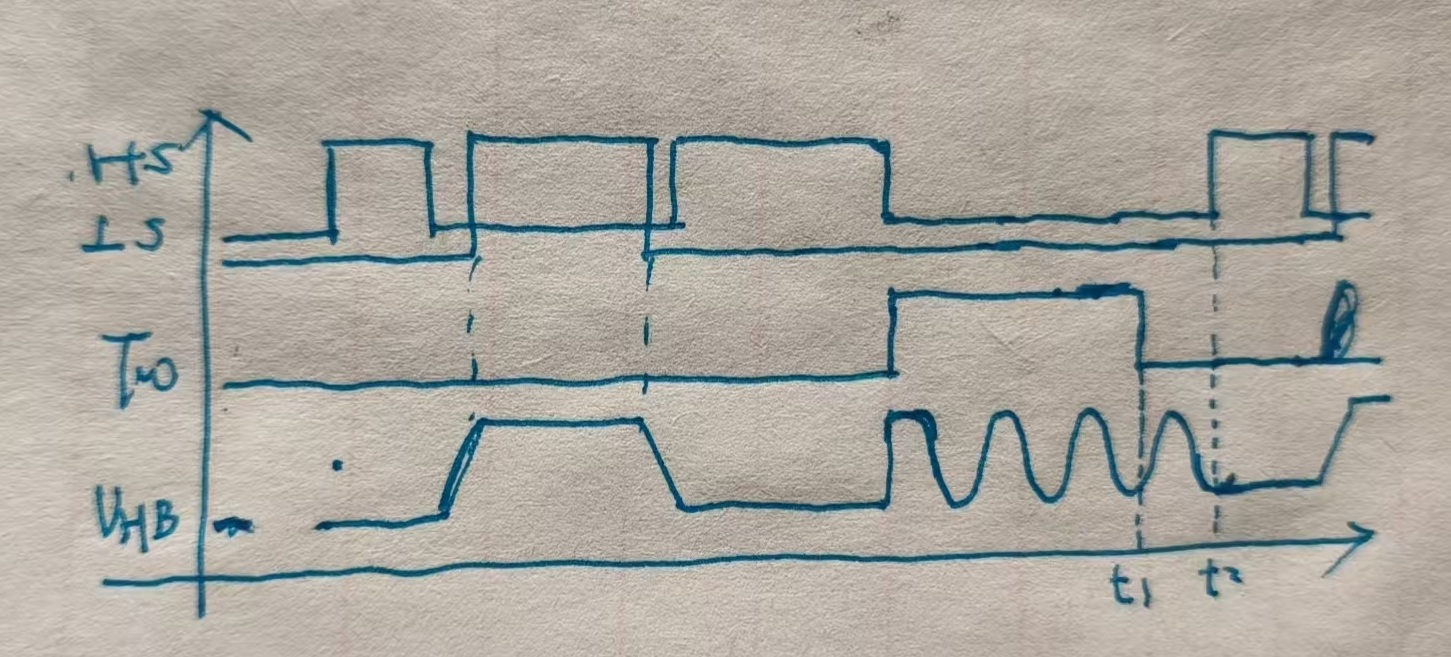
\includegraphics[width=0.6\linewidth]{figures/谷值锁定波形1.jpg}
    \caption{谷值锁定波形1}
    \label{fig:谷值锁定波形1}
\end{figure} 

若使用随负载变化控制频率大小的振荡器电路来产生$T_w$,可能会出现在功率重叠范围内即使输出负载不变,$T_w$内信号$V_{HB}$的谐振谷数值在不同开关周期内发生来回跳动的情况,称之为跳谷现象,为解决该问题,设计了谷值锁定电路。

谷值锁定电路的作用同样是根据负载的轻重情况调节开关频率大小,副边反馈引脚电压信号$V_{FB}$如~\ref{sec:峰值电流控制电路}小节中提到的,是峰值电流参考电压$V_{CSP}$的重要组成部分,可以一定程度地反映输出负载电流的大小。为了降低导通损耗,需要维持一个较低的峰值电流,因此在负载变化时,利用谷值锁定电路根据$V_{FB}$的变化动态调节谐振谷的数量,以改变$T_w$时间长度的方式改变开关频率,更快地恢复输出电压的稳定。
但不同与振荡器电路的是,为了防止跳谷现象的产生,通过对负载的变化调整并锁定等待时间$T_w$内的谐振谷数值,只有当电路判断实际的谷值和设定谷值相等时,才允许精确谷底导通模块在最近的谷底处导通低边功率管,开启下一开关周期。该电路彻底避免了在负载不变的情况下谐振谷值的频繁变化问题,减小了电路的不稳定现象。

谷值锁定电路具体组成如图~\ref{fig:谷值锁定电路1}所示,主要包括三个迟滞比较器、一个D触发器、一个单向计数器、一个双向计数器和DAC电路等。
%该电路的设计原理是,当输出负载电流较小时,$V_{FB}$的电压值也较小,此时谷值锁定电路增大$T_w$时间内的谐振谷值,降低开关频率。

\begin{figure}[htbp] 
    \centering
    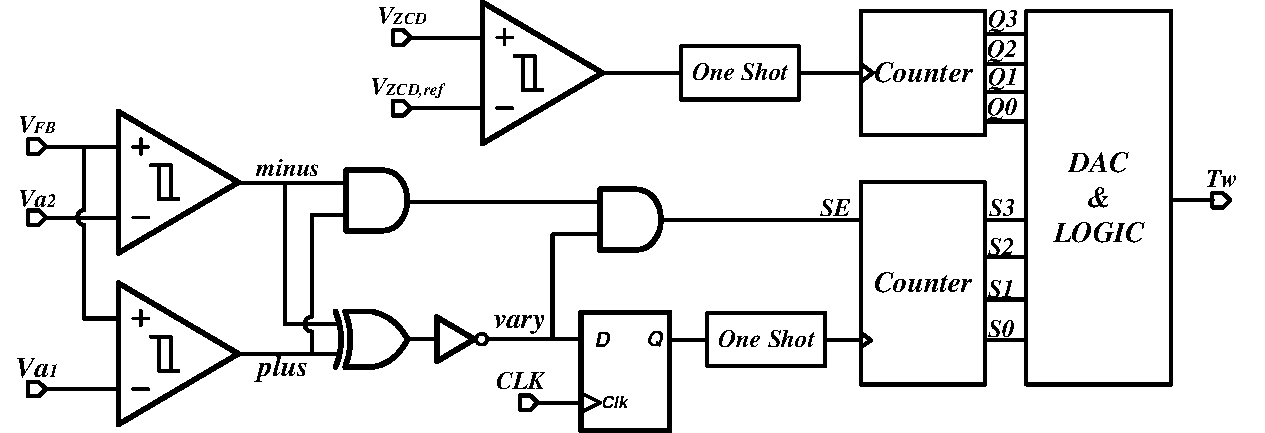
\includegraphics[width=0.8\linewidth]{figures/谷值锁定电路1.pdf}
    \caption{谷值锁定电路1}
    \label{fig:谷值锁定电路1}
\end{figure} 

如图~\ref{fig:谷值变化策略}的谐振谷数值变化策略所示,当输出负载电流较小时,$V_{FB}$电压值小于参考电压Va1,比较器3的输出端plus等于逻辑“1”,此时需要随着CLK信号的触发通过双向计数器电路增加$T_w$时间内的谐振谷数量,降低开关频率;当输出负载电流较大时,$V_{FB}$电压值大于参考电压Va2,比较器2的输出端minus等于逻辑“1”,说明需要减小$T_w$时间内的谐振谷数量,增大开关频率;当$V_{FB}$大于Va1但小于Va2时,锁定$T_w$时间内的谐振谷数量,防止发生跳谷现象。

\begin{figure}[htbp] 
    \centering
    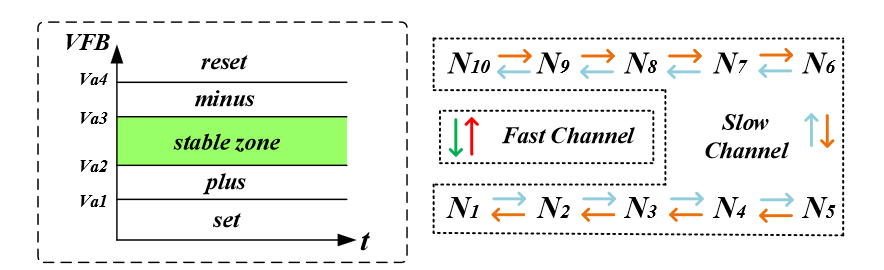
\includegraphics[width=0.8\linewidth]{figures/谷值变化策略.png}
    \caption{谷值变化策略图}
    \label{fig:谷值变化策略}
\end{figure} 

信号$V_{FB}$和参考电压Va1、Va2通过比较器比较后输出的信号plus、minus的组合逻辑决定了谷值锁定电路不同的工作状态,具体工作状态如~\ref{tab:谷值锁定电路}表所示。如在plus信号为逻辑“0”,minus信号为逻辑“1”时,谷值锁定电路将对谐振谷数量进行锁定;在plus和minus信号的其他逻辑转态将对谐振谷进行增加或减小数量的调整操作。plus和minus信号通过一个同或门后输出vary信号并连接到D触发器的D输入端,保证在vary信号为逻辑“1”时允许时钟信号CLK对双向计数器进行计数。plus和minus信号还经过两个与门后输出SE信号,SE信号控制了双向计数器向上和向下的两种计数模式。当SE信号为逻辑“1”时,双向计数器进行向上计数操作,增加$T_w$时间内的谐振谷数量;当SE信号为逻辑“0”时,双向计数器进行向下计数操作,减少$T_w$时间内的谐振谷数量。双向计数器输出的4bit信号S[3:0]会通过DAC电路转为模拟电压信号,与另一个计数器产生的4bit信号Q[3:0]产生的电压信号进行比较,输出$T_w$等待时间给精确谷底导通电路。


%为了防止出现如前文~\ref{sec:多模式切换}小节中提到的峰值电流和开关频率同时变化引起的相位裕度降低和电路不稳定情况,轻载时采取的RVS工作模式通过改变开关频率的方式维持峰值电流的基本恒定。副边反馈引脚电压信号$V_{FB}$如~\ref{sec:峰值电流控制电路}小节中提到的,是峰值电流参考电压$V_{CSP}$的重要组成部分,可以一定程度地反映输出负载电流的大小。当负载电流突然增大时,为了满足变大的输出功率,变压器原边需要增大高边功率管的导通时间提供更多的能量给输出电容,因此$V_{CSP}$增大,$V_{FB}$也相应地增大;当负载电流突然减小时,同理$V_{FB}$也会相应地减小。同时为了降低导通损耗,需要维持一个较低的峰值电流,因此在负载波动时,利用谷值锁定电路通过随$V_{FB}$变化动态调节谐振谷的数量,改变$T_w$时间长度的方式改变开关频率,更快地恢复输出电压的稳定。



\begin{table}[htbp]
    \caption{谷值锁定的三种操作}
    \label{tab:谷值锁定电路}
    \centering
    \belowrulesep=0pt  %防止竖线不连续
    \aboverulesep=0pt  %防止竖线不连续
        \begin{tabular}{|c|c|c|c|c|}
            \toprule
             (minus,plus) & 功能 & vary & SE \\
            \midrule
             (0,0)  & 减小谷值  & 1 &    0                   \\  \midrule
             (0,1)  & 锁定谷值  & 0 & disable                \\  \midrule
             (1,1)  & 增加谷值  & 1 &    1       \\          
            \bottomrule
        \end{tabular}
\end{table}

4bit双向计数器电路的电路图如图~\ref{fig:双向计数器电路}所示,包括四个D触发器和MUX电路。不同于普通的单向计数器,可以通过SE信号选择实现向上或向下计数的功能。当SE信号为逻辑“1”时,将每个D触发器的反向输出端输入到下一个D触发器的CLK输入端,此时是向上计数功能;当SE信号为逻辑“0”时,MUX将D触发器的正向输出端输入到下一个D触发器的CLK输入端,实现向下计数功能。电路中还包括hold信号,hold信号的作用是消隐掉SE信号的电平切换的上升沿或下降沿,防止其对计数方向切换造成影响。

\begin{figure}[htbp] 
    \centering
    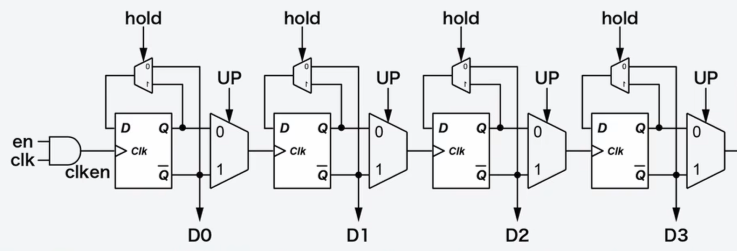
\includegraphics[width=0.8\linewidth]{figures/双向计数器电路.png}
    \caption{双向计数器电路图}
    \label{fig:双向计数器电路}
\end{figure} 

谷值锁定电路中的DAC电路如图~\ref{fig:双向计数器电路}所示,计数器的计数值作为DAC的输入信号,两个计数器分别控制思路电流镜开关管的导通和关断,每个电流镜的镜像比例为1:2:4:8,成倍增加,产生随4bit数字信号S[3:0]、Q[3:0]信号对应的电流$I_S$、$I_Q$。电流镜采用了cascode结构增大电流镜的输出阻抗,提高电流镜像的精度。每一路电流镜还都添加了毛刺消除结构晶体管M11、M13等,用于吸收当数字信号控制M10、M12等开关管导通瞬间产生的巨大毛刺电压。
没有毛刺消除结构时,如图~\ref{fig:双向计数器电路}中的电压V2和V3,分别为晶体管M2和M3的漏极电压,在数字信号S0未导通开关管M10时,$V_2=V_3=V_{DD}$;当S0控制开关管M10导通,电压V3由于cascode结构的大输出阻抗的作用下和电压V1近似相等,电压V2则由于开关管导通等于电阻$R_S$上的电压。在开关管通断前后电压V2和V3的变化量分别为:
\begin{equation}
    \label{eq:△V2公式}
    \varDelta V_2 = V_{DD} - V_{GS1}
\end{equation}
\begin{equation}
    \label{eq:△V3公式}
    \varDelta V_3 = V_{DD} - V_S
\end{equation}

由于电流镜晶体管存在寄生电容$C_{ds}$,故电流镜晶体管M3和M2的寄生电容上的能量$\varDelta P_3 = \varDelta V_3 C_{ds3}$、$\varDelta P_2 = \varDelta V_2 C_{ds2}$会在开关管导通的瞬间传递到电阻$R_S$上,在电压$V_S$引起巨大的毛刺。加入毛刺消除结构M11后,由于M11是NMOS晶体管,其会和开关管M10交替导通,在晶体管M11导通时,电压V2等于零,电压V3的值仍近似等于V1;当开关管M10导通的时候,电压V2和V3的值和没有晶体管M11时相同,故电压V2和V3的变化量分别变为:
\begin{equation}
    \label{eq:△V2公式1}
    \varDelta V_2 = V_{GS1} - V_{GS1} = 0
\end{equation}
\begin{equation}
    \label{eq:△V3公式1}
    \varDelta V_3 = V_S - 0 = V_S
\end{equation}
由式中可见得,电压V2和V3的变化量大大降低,明显降低了毛刺现象。

\begin{figure}[htbp] 
    \centering
    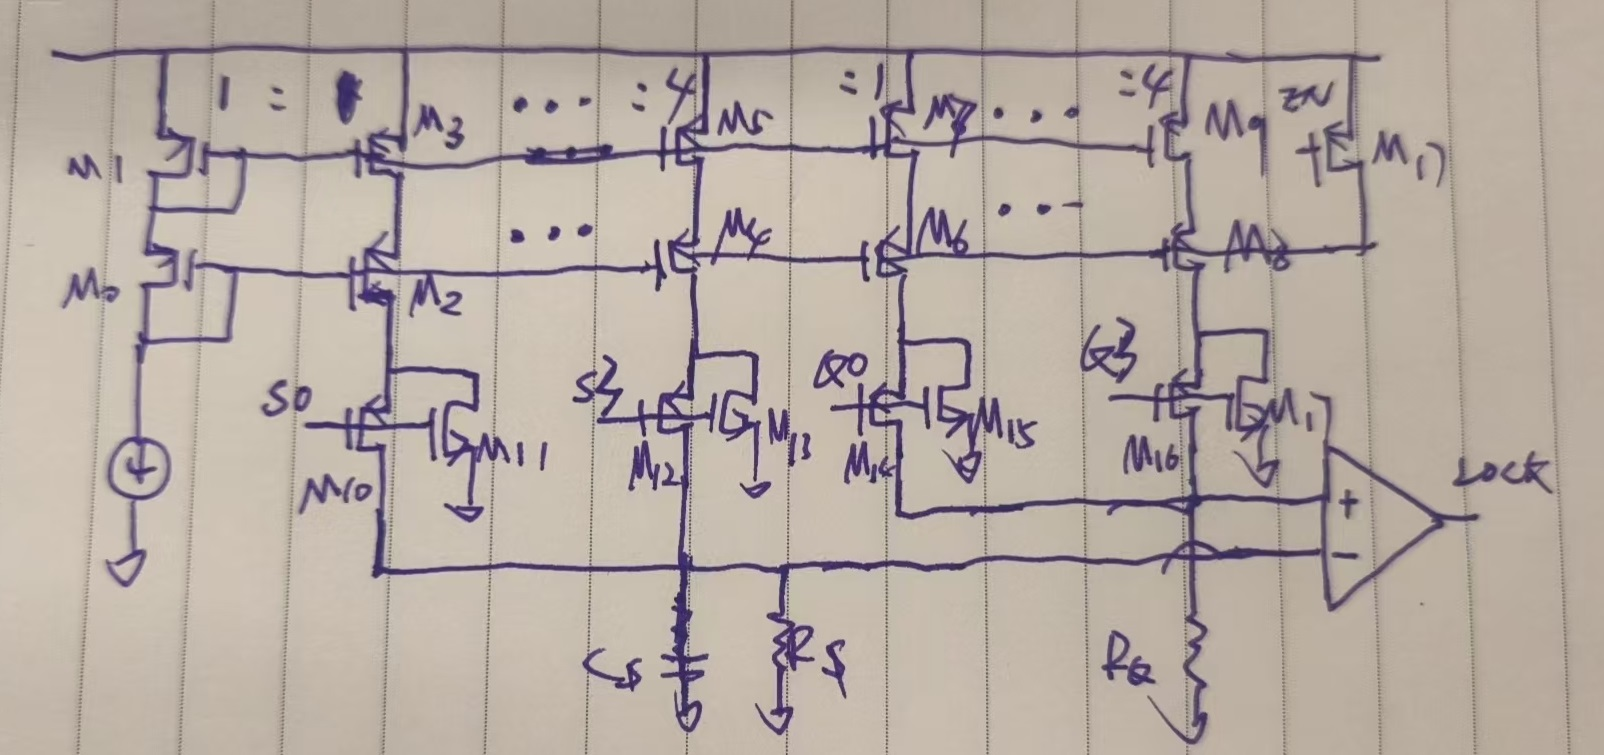
\includegraphics[width=0.6\linewidth]{figures/DAC电路.jpg}
    \caption{DAC电路图}
    \label{fig:DAC电路}
\end{figure} 

数字信号S[3:0]、Q[3:0]控制产生的电流$I_S$、$I_Q$流经电阻$R_S$、$R_Q$后产生的电压$V_S$、$V_Q$通过比较器进行比较大小,当电压$V_Q$大于$V_S$后,比较器输出信号$T_w$由高电平转为低电平,锁定时间结束,精确谷底导通电路开始工作,寻找最近的谐振谷底开启下一开关周期。

\begin{figure}[htbp] 
    \centering
    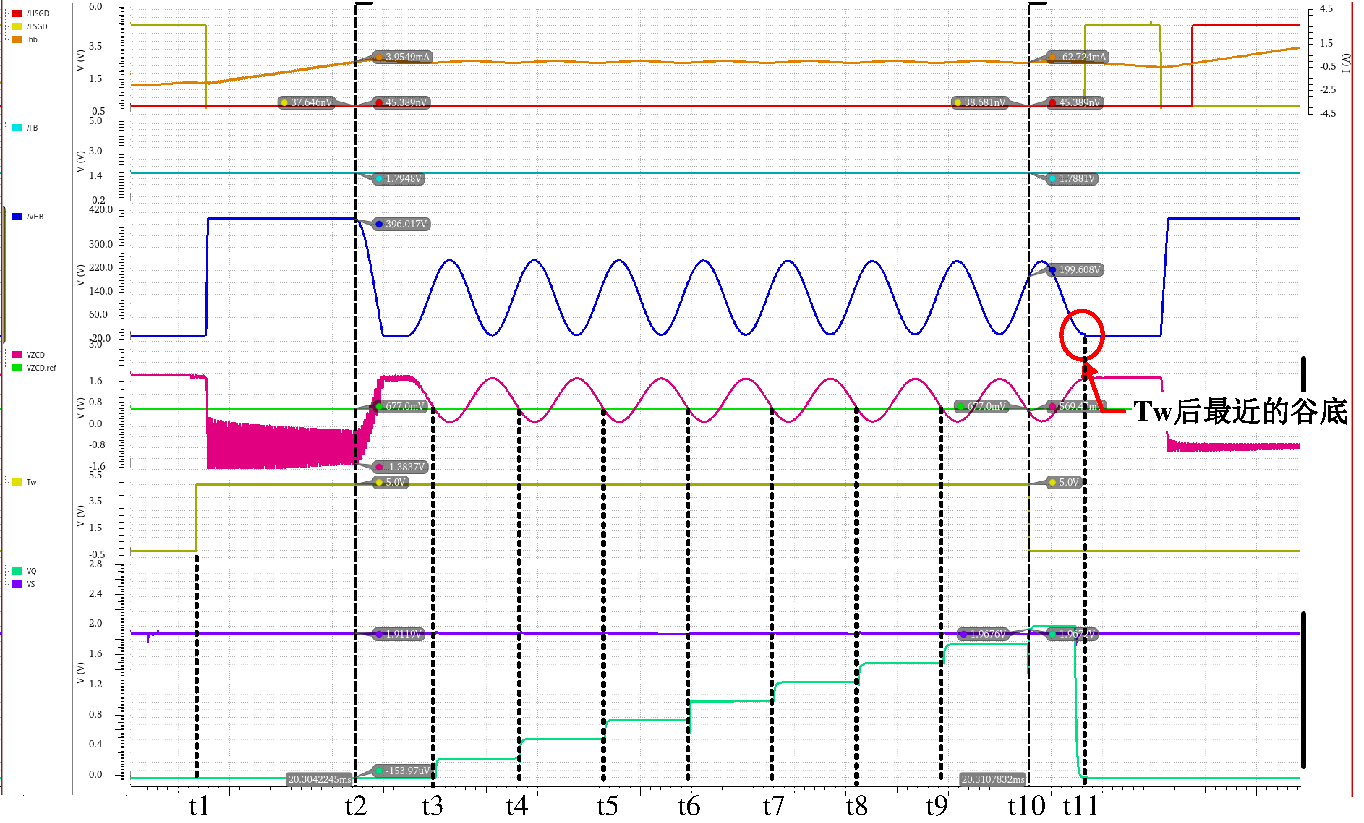
\includegraphics[width=0.8\linewidth]{figures/valley_lock.pdf}
    \caption{谷值锁定电路波形图}
    \label{fig:valley_lock}
\end{figure} 

\section{逻辑控制电路}

\section{保护电路}

\section{系统整体仿真}

\section{小结}




